\documentclass[10pt,a4paper]{article}
\usepackage[a4paper, total={7in, 8in}]{geometry}

\usepackage[utf8]{inputenc}
\usepackage[T1]{fontenc}
\usepackage[export]{adjustbox}
\usepackage[french]{babel}
\usepackage{graphicx}
\usepackage{eso-pic}
\usepackage{transparent}
\usepackage[export]{adjustbox}
\usepackage{hyperref} \hypersetup{colorlinks, citecolor=black, filecolor=black, linkcolor=black, urlcolor=black,}
\usepackage[nonumberlist]{glossaries}
\usepackage{glossaries}
\usepackage{imakeidx}

% 1 : Logo ulb en fond
\newcommand\BackgroundPic{%
    \put(0,-47){%
        \parbox[b][\paperheight]{\paperwidth}{%
            \vfill
            \centering
            {\transparent{0.09}
\includegraphics[width=1.17 \textwidth]{Fondulb.jpg}}%
            \vfill
        }
    }
}





% Glossaire
\newglossaryentry{Tower Defense}
{
  name=Tower Defense,
    description={Jeu de stratégie où le but est de défendre la zone d'un \gls{joueur} contre des vagues  successives d'\glspl{ennemi}\index{ennemi} en construisant et en améliorant progressivement ses tours.}
}
\newglossaryentry{joueur}
{
  name=joueur,
    description={Personnage fictif du jeux qu'incarne l'\gls{utilisateur}}
}

\newglossaryentry{utilisateur}
{
  name=utilisateur,
    description={Personnage réel qui joue à Meatwars: Revenge of the Falling Vegan}
}

\newglossaryentry{compte}
{
  name=compte,
    description={Contient toutes les données de l'\gls{utilisateur}}
}

\newglossaryentry{serveur}
{
  name=serveur,
    description={Programme qui réceptionne les connections des \glspl{client}. Il a les données de tous les \glspl{utilisateur}}
}

\newglossaryentry{client}
{
  name=client,
    description={Programme que l'\gls{utilisateur} lance pour se connecter au \gls{serveur}. Il permet à l'\gls{utilisateur} de jouer au jeu via le terminal ou l'interface graphique}
}

\newglossaryentry{ennemi}
{
  name=ennemi,
  description={Personnage fictif qui apparaît avec intervalle régulier dans une vague qui a un certain niveau de vie.}
}

\newglossaryentry{argent}
{
  name=argent,
  description = {Monnaie qui permet au \gsl{joueur} de s'acheter des \gls{tours} pour permettre de résister aux vagues d'\glspl{ennemi}.}
}

\newglossaryentry{tours}
{
  name=tours,
  description={Objet de défense permettant à un joueur de contrer les vagues d'\glspl{ennemi}, à  chaque \gls{ennemi} détruit le \gls{joueur} gagne de la \gls{argent}.Une \gsl{tours} coûte 200 .}
}

\newglossaryentry{map}
{
  name= map,
  description={Espace représentant le plateau de jeu avec lequel les joueurs pourront avoir des interactions(placer des \gls{tours} sur les partie délimité par des \# et montreras aussi le déplacement des \glspl{ennemi} selon des chemins prédéfinies.}
}

\newglossaryentry{supporter}{
    name= supporter,
    description={Personnage fictif que l'\gls{utilisateur} qui ne peut peut jouer une partie mais peut intervenir en donnant de l'\gls{argent} à un \gls{joueur} ou plusieurs.}
}
\makeglossaries
\setglossarysection{subsection}


\makeindex
\indexsetup{level=\chapter}
% Pour ajouter un mot à l'index: "\index{mot}"



\begin{document}
\AddToShipoutPicture*{\BackgroundPic}

\begin{titlepage}
\begin{center}
\vspace*{-1.5cm}

\includegraphics[width=8cm]{ulb.pdf}
\vspace{6cm}

\par{\huge \textbf{SRD: Tower Defense}}\bigbreak
\bigbreak
\par{\huge \textbf{\textit{{Meat war: Rise of the fallen vegan}}}}
\vspace{2cm}
\par{\large [Cours: INFO-F-209]}
\vspace{2cm}

\par \hrulefill \par
\vspace{1cm}
\bsc{Jacobs} Alexandre 
\bsc{\&}
\bsc{Innocent} Antoine
\bsc{\&}
\bsc{André} Bob
\bsc{\&}
\bsc{Vangeem} Nicolas
\bsc{\&}
\bsc{Roos} Kim
\bsc{\&}
\bsc{Paquet} Michael
\bsc{\&}
\bsc{Singh} Sundeep
{\emph \\BA2 Informatique}
\vspace{0.7cm}
\par \hrulefill \par

\vspace{2cm}
\par Mars 2017

\end{center}
\end{titlepage}
\newpage
\tableofcontents
\newpage

\section{Introduction}
\subsection{But du projet}
 Notre projet consiste en une réalisation d'un \index{\gls{Tower Defense}} qui sera jouable en réseau sous Linux. Il est aussi de permettre aux étudiants de mettre en pratique les différents concept vus dans les cours de système d'exploitation et d' analyse et méthodologie informatiques. De plus, le respect de conventions de codage, du paradigme orienté-objet et l'analyse UML faites seront un aspect essentiel à la réalisation de notre projet.  


Ce document joue le rôle du document de spécification des besoins, SRD (System requirement Document) pour le projet INFO-F209 : "Meat war: Rise of the falling vegan".
  Ces exigences portent sur un travail de groupe (8 personnes) codé majoritairement en C++ avec une section C pour le \gls{serveur} \index{serveur}. Le produit final est donc un jeu de type \gls{Tower Defense} \index{Tower Defense} multijoueur en réseau.
Ce jeu n'ayant aucun but lucratif, nous considérons le \index{\gls{client}} principal comme étant le \gls{joueur}\index{joueur} du jeux en question.
Ainsi, ce document présente des spécifications propres à l'\gls{utilisateur}\index{utilisateur} et propre au système. Celui-ci va également mettre en avant la communication \gls{client} \index{client}/ \gls{serveur} \index{serveur} afin de bien mettre en place l'aspect multijoueur réseau du produit. 


 Ce document ne varie pas en fonction des différentes architectures ou systèmes d'exploitation.

\subsection{Présentation du jeu}
 Le nom de notre projet est "Meat war: Rise of the fallen vegan".
Lors d'une création de \gls{compte}\index{compte}, chaque \gls{utilisateur}\index{utilisateur} reçoit une certaine somme d' \glspl{argent} \index{argent} qui lui permettra d'acheter des \gls{tours} \index{tours} lors des parties.
\noindent Lors de partie, chaque \gls{joueur}\index{joueur} se voit attribuer une partie de la \gls{map}\index{map}. Chaque \gls{joueur}\index{joueur} utilisant à sa guise la partie de la \gls{map}\index{map} lui ayant été attribué. Par ailleurs, les termes utilisé et lié au jeu ont été choisis en fonction du thème que nous sommes imposés.

% Glossaire
\glsaddall
\printglossary[numberedsection]

\subsection{Historique de document}

\begin{center}
\hspace*{0cm}
\begin{tabular}{|c|c|c|c|}
\hline
Versions & Auteur & Date & Modifications \\
\hline
2.0 & Équipe & 05-03-2017 &\textbf{Deadline pour la phase 2}\\
1.5 & Alexandre & 05-03-2017 & Mise à jour diagramme UML\\
1.4 & Alexandre & 28-02-2017 & Révision besoin système \& utilisateur.\\
1.3 & Alexandre & 28-02-2017 & Ajout de certains termes.\\
1.2 & Alexandre & 27-02-2017 & Modification de la section Introduction.\\
1.1 & Antoine \& Bob & 10-02-2016 & Correction suite à de la réunion du 06-02-2017. \\
1.0 & Équipe & 19-12-2016 & \textbf{Deadline pour la phase 1}\\
0.3 & Kim & 16-12-2016 & Ajout du glossaire et de l'index\\
0.2 & Équipe & 16-12-2016 & Ajout des besoins d'utilisateur et besoins du système.\\
0.1 & Sundeep \& Michael & 10-12-2016 & Ajout des use cases et diagrammes d'activité au niveau utilisateur.\\
0.0 & Alexandre \& Antoine & 10-12-2016 & Création de la structure du document.\\
\hline
\end{tabular}
\end{center}


\newpage
\section{Besoins de l'utilisateur}

 Les besoins de l'\gls{utilisateur}\index{utilisateur} seront expliqués au travers de plusieurs graphes/explications, en voici ici un résumé.\\
Le but de l'application est de permettre à l'\gls{utilisateur}\index{utilisateur} de pouvoir jouer à un jeu de type \gls{Tower Defense} \index{Tower Defense}. Celui-ci sera disponible depuis un menu\index{menu} accessible après connexion et offrira au \gls{utilisateur}\index{utilisateur} plusieurs services. En effet, l'\gls{utilisateur}\index{utilisateur} devra se créer un \gls{compte}\index{compte} avant d'avoir accès au menu.\\
Il pourra alors consulter son profil\index{consulter son profil}.
Un classement\index{classement} sera également accessible et permettra de situer un \gls{joueur}\index{joueur} par rapport à un autre en fonction de leur score respectif.\\
Comme dit implicitement plus haut, l'\gls{utilisateur}\index{utilisateur} disposera d'une liste d'amis\index{liste d'amis} qui pourra modifier(ajouter, supprimer et accepter des demandes d'amis) et afficher sa liste d'amis.\\

 Le menu\index{menu} permettra bien évidemment à un \gls{utilisateur}\index{utilisateur} premièrement de se connecter à un \gls{compte}\index{compte} déjà existant ou de se créer un \gls{compte}\index{compte}, deuxièmement une fois l'\gls{utilisateur}\index{utilisateur} connecté, ce dernier pourra décider de démarrer une partie, donc de choisir un mode de jeu pour qui ouvrira un salon en attendant d'avoir le nombre requis de \glspl{joueur} afin de jouer une partie. Mode, et nombre de \glspl{joueur}\index{joueur} (au maximum de 4) seront spécifiés par le \gls{client} avant que celui-ci ne lance la partie\index{partie}. Il pourra aussi rejoindre une partie en tant que \gsl{supporter}\index{supporter}, afficher son profil et gérer ses amis. Une seule et unique carte sera cependant disponible.
\subsection{Exigences fonctionnelles}
\subsubsection{Use case: menu\index{menu}}
\begin{center}
    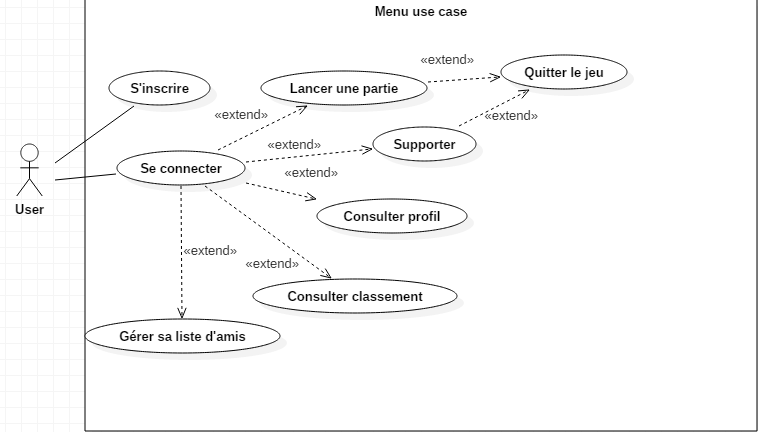
\includegraphics[height=12cm,width=16.45cm]{menu_use_case.png}
\end{center}
\par
%\newpage
\begin{itemize}
\item \textit{\textbf{Acteurs}} : ce use case a comme  1 acteur acteur qui est l'\gls{utilisateur}\index{utilisateur}.\\

\item \textit{\textbf{Pré-conditions}} : il y en a 2 , à savoir que le \gls{utilisateur}\index{utilisateur} se soit connecté, si c'est un nouvel utilisateur doit d'abord s'inscrire puis se connecter.\\

\item \textit{\textbf{Post-conditions}} : il y a deux post-conditions. Soit le menu\index{menu} est quitté et donc le \gls{joueur}\index{joueur} est déconnecté, soit le \gls{joueur} a lancé une partie\index{partie}, rejoint une partie en tant que supporter, consulter son profil ou gérer sa liste d'amis.\\

\item \textit{\textbf{Flux d'exécution}} : en ce qui concerne le flux d'exécution basique, le \gls{joueur} va d'abord se connecter. Une fois connecté, il peut lancer une partie\index{partie}, consulter son profil, son classement et gérer ses amis. Finalement, avant de lancer une partie\index{partie}, il peut choisir le mode de jeu.

\end{itemize}    

 \subsubsection{Diagramme d'activité du menu:}

 \begin{center}
 
     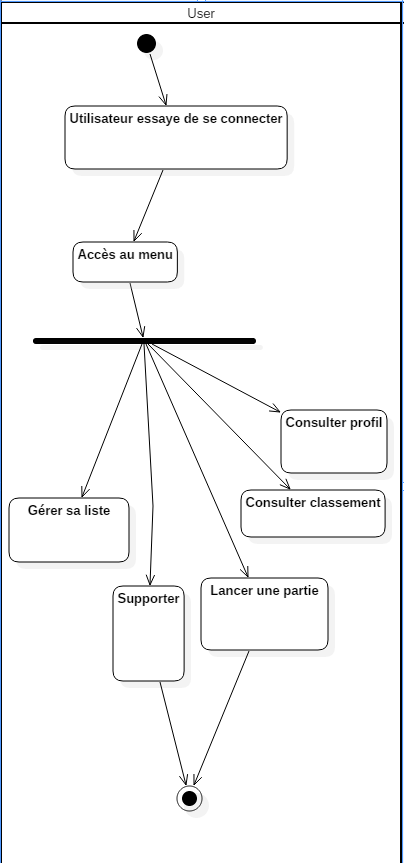
\includegraphics[height=17cm,width=10cm]{user_serveur_diagramme.png}
 
 \end{center}
   
\newpage
\subsection{Use case: en jeu}

\subsubsection{Use case diagramme en jeu:}

\begin{center}
    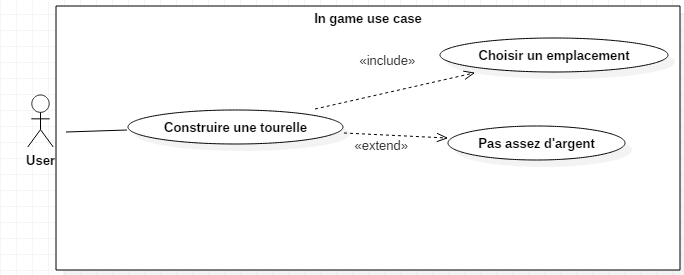
\includegraphics[height=13.5cm,width=17cm]{ingame_use_case.png}
\end{center}

%\newpage
\begin{itemize}
\item \textit{\textbf{Acteurs}} : ce use case a comme unique et principal acteur le \gls{joueur}\index{joueur}.\\

\item \textit{\textbf{Pré-conditions}} : pour ce qui est des pré-conditions le \gls{joueur} doit être connecté et a dû lancer une partie\index{partie}.\\

\item \textit{\textbf{Post-conditions}} : la seule post-condition est qu'une fois la partie\index{partie} terminée, le \gls{joueur} retourne au menu\index{menu}.\\

\item \textit{\textbf{Flux d'exécution}} : pour ce qui est du déroulement basique, une fois en jeu le \gls{joueur}\index{joueur} peut construire des tourelles, consulter la description de celles-ci, il peut également les améliorer, les vendre, mais aussi modifier les paramètres du jeu. Il existe également un flux d'exécution alternatif. Au lieu de jouer, l'\gls{utilisateur}\index{utilisateur} peut être tout simplement un spectateur de la partie\index{partie}.

\end{itemize}


\newpage
\subsubsection{Diagramme d'activité lors que le joueur est en jeu:}

\begin{center}
    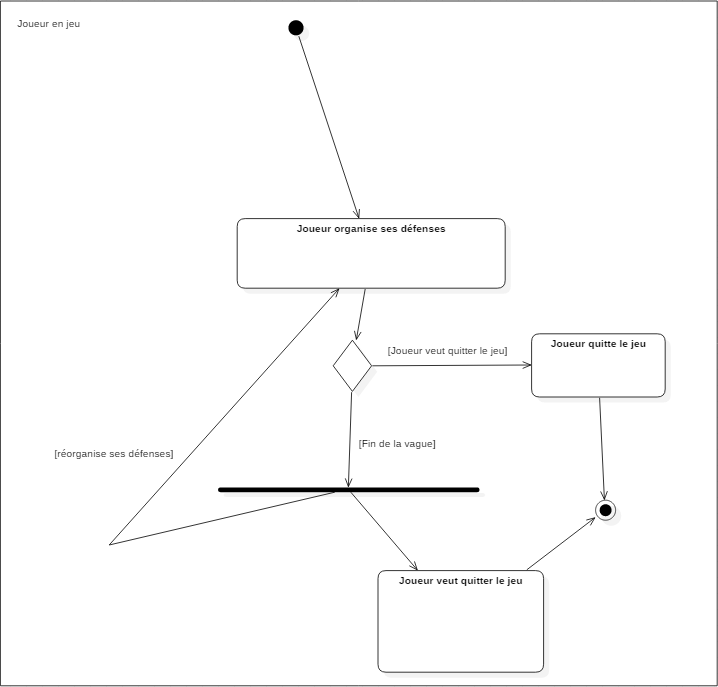
\includegraphics[height=16cm,width=19cm]{joueur_en_jeu.png}
\end{center}

\newpage    
\subsection{Exigences non fonctionnelles}

\begin{itemize}
    \item Menu\index{menu} et interface intuitifs.
    \item Animations graphiques.
    \item Maniabilité
    
\end{itemize}
    
\subsection{Exigence de domaine}

\begin{itemize}
  \item Le jeu doit être multijoueur, les différents \glspl{utilisateur}\index{utilisateur} connectés sur un même \gls{serveur}\index{serveur} doivent pouvoir agir sur le terrain.
   \item  L'abandon\index{abandon} d'un des \glspl{joueur}\index{joueur} ne doit pas empêcher les autres de terminer leur partie\index{partie}. 
   \item Un jeu de \gls{Tower Defense}\index{Tower Defense} est un jeu de 2 à 4 \glspl{joueur}\index{joueur} qui ont chacun une partie\index{partie} de la carte.
   \item Chacun des \glspl{joueur}\index{joueur} a sa base\index{base} dans chaque coin du jeu.
   \item Les \glspl{ennemi}\index{ennemi} apparaissent au milieu de la carte, leur vagues sont identiques pour chaque \gls{joueur}.
   \item La partie\index{partie} se déroule sous forme de vagues successives d’\glspl{ennemi}\index{ennemi} jusqu’à ce que la partie\index{partie} se termine.
   \item  Les \glspl{joueur}\index{joueur} peuvent améliorer ou acheter des tours à tout moment de la partie\index{partie}.
   \item  La partie se termine si le temps est écoulé dans le cas d’une partie\index{partie} en mode chrono\index{mode chrono} ou s’il ne reste que un \gls{joueur} vivant dans le cas d’une partie classique\index{partie classique}.
\end{itemize}
\newpage
\section{Besoin du système}
\subsection{Exigences fonctionnelles}
Les exigences fonctionnels du système regroupent les besoins explicité par le
clients qui ont une conséquences sur l'architecture du système. Ces exigences
n’ont aucun lien avec l’utilisateur et sont donc implicites.
Après avoir analysé les exigences, on a pu déterminer donc plusieurs exigences fonctionnels: \\

\begin{itemize}
    \item Démarrer\&Initier une partie\index{partie}:\
    Fonction qui initie une \index{partie} lorsqu'un \gls{utilisateur}\index{utilisateur} en fait la demande. Pour cela différentes données sont nécessaires tels que le mode de jeux et le nombres de \glspl{joueur}\index{joueur} requis pour la partie\index{partie}. Une fois le nombre atteint la partie \index{partie}, le serveur lance automatiquement la partie chez tout les \glspl{utilisateur} et rafraîchit leur interface.
    \item Trouver une partie \index{partie}: Lorsqu'un \gls{utilisateur} veut jouer une partie ou en rejoindre une pour être supporter, le serveur fait appel au matchmaking qui permet de regrouper plusieurs personnes dans un même salon de jeu, en attendant le début d'une partie. 
    \item Partie:
    Cela est une composante importante du programme. La \index{partie} se compose de divers fonctionnalités: placer une tours, vérification de victoire, défaite et établissement des scores et récompenses attribuer à chaque à \gls{joueur}.
    \item Classement: Regroupe tout les scores des joueurs classé du meilleur au moins bon score et est mis à jours après chaque partie.
\end{itemize}

\subsection{Exigences non fonctionnelles}
Les exigences non-fonctionnels reprennent l’ensemble des exigences qui sont compris comme important afin de réaliser correctement
le projet. Dans cette section, nous reprenons donc donc les quelques aspect qui ont pas été
exprimés de manière explicite par le client.
Par ailleurs, il est évident que un certains nombre d’interactions entre le \gls{client}\index{client} et le \gls{serveur}\index{serveur} seront mises en place, vu que le projet est un programme devant être jouable en réseau.\\


\begin{itemize}
    \item Création d'un \gls{compte}\index{compte} \gls{utilisateur}\index{utilisateur} et connexion de celui-ci au système.
    \item Mise à jour des amis d'un joueur. 
    \item Organisation.
    \item Réactivité.
\end{itemize}
\\
De plus, les différents points, qui sont repris ci dessus, ne reflètent les aspects clés qui ont été déterminé suite à la rencontre avec le client.\\
%\newpage
\subsection{Design et fonctionnement du système}
Cette sections reprends les diagrammes permettant de décrire l'architecture du système et son fonctionnement. Les différents diagrammes UML ayant été utilisé sont diagrammes de classe, de séquence et d'activité.
  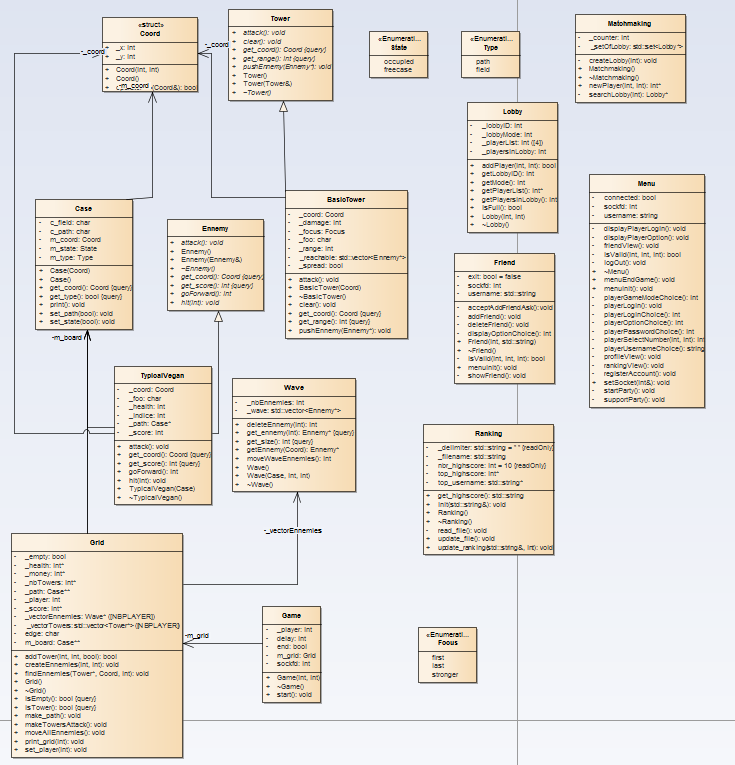
\includegraphics[height=20cm,width=20cm]{classe_diagramme.PNG}
\newpage
\subsubsection{Diagramme de sequence d'une connection}
  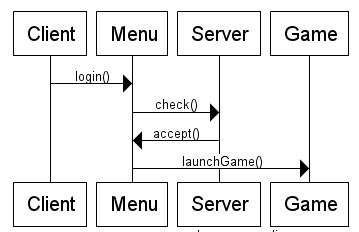
\includegraphics[height=9.5cm,width=16cm]{sequence.png} 

\newpage


%\section{Index et termes utilisés}
\printindex

\end{document}
